\chapter{Introdução}
\label{ch:introducao}
\begin{resumocapitulo}
	No capítulo a seguir, iremos abordar o consumo do café nas regiões Metropolitanas de São Paulo com a utilização de técnicas  avançadas em machine learning em conjunto em analises exploratórias. A análise inclui os benefícios do café para a saúde, a importância econômica do café em São Paulo, a industrialização impulsionada pelo café e a aplicação de modelos de machine learning para prever o preço do café, analisar nivel de  consumido por território e tipos de café existente.  
 % \href{http://docs.uninove.br/arte/pdfs/Manual_de_Trabalhos_Academicos_ABNT_UNINOVE.pdf}{clique aqui.}
\end{resumocapitulo}

\section{Benefícios do Café para a Saúde } 
\label{sec:Benefícios do Café para a Saúde}O consumo de café tem sido
amplamente estudado devido aos seus efeitos na saúde. Segundo uma pesquisa, o café possui uma complexa composição química que inclui cafeína e outros compostos bioativos que podem oferecer vários benefícios à saúde. Estudos indicam que o consumo moderado de café está associado à redução do risco de doenças como Parkinson e Alzheimer, além de melhorias no desempenho cognitivo e no humor. \cite{alves2009beneficios}

\section{Importância Econômica do Café no Brasil }
\label{sec:Importância Econômica do Café no Brasil}
O café é um dos principais produtos agrícolas do Brasil, desempenhando um papel crucial na economia do país. A história do café no Brasil está intimamente ligada ao desenvolvimento econômico e social do país. O setor cafeeiro brasileiro enfrenta desafios constantes, como a variabilidade dos preços e as condições climáticas adversas, que afetam diretamente a produção e a exportação do café. \cite{lopes2018prediccao}

\section{Previsão de Preços do Café com Machine Learning }
\label{sec:Previsão de Preços do Café com Machine Learning}
A previsão de preços de commodities agrícolas, como o café, é vital para a tomada de decisões por parte dos produtores. Um estudo utilizou modelos de machine learning, incluindo Support Vector Machine (SVM), LASSO e Random Forest, para prever os preços do café brasileiro. Entre os modelos analisados, o SVM com kernel linear apresentou o melhor desempenho preditivo. Essa abordagem não só melhora a precisão das previsões de preços, mas também auxilia na gestão de riscos e controle por parte dos administradores \cite{lopes2018prediccao}.

\subsection{Industrialização e o Café}
\label{Industrialização e o Café}
A relação entre o café e a industrialização de São Paulo é um ponto central na história econômica brasileira. Fernando Henrique Cardoso argumenta que o surto de industrialização da cidade foi em grande parte impulsionado pelo café, que forneceu o capital necessário para o desenvolvimento industrial segundo   \citeonline{cardoso1960cafe} (Revistas USP). Esta perspectiva destaca como a economia cafeeira foi fundamental para a transição econômica e social do Brasil, transformando São Paulo em um centro industrial. 

\subsection{Hábitos em Mudança}
\label{subsec:citacao_indireta}
A pesquisa da ABIC e do Instituto Axxus, realizada entre 2019 e 2023 com 4.200 pessoas, aponta mudanças significativas no comportamento do consumidor de café no Brasil (ABIC, 2023). Em 2021, o consumo em casa era predominante devido à pandemia, mas em 2023, com o fim das restrições, o trabalho voltou a ser o principal local de consumo, seguido pelo lar (ABIC, 2023).
Perfil do Consumidor:
-Consumo: 29 dos consumidores ingerem mais de seis xícaras de café por dia, enquanto 46 consomem entre três e cinco (ABIC, 2023).
-Momento do Dia: 97 preferem o café ao acordar e 88 o consomem durante a manhã (ABIC, 2023).
-Motivações: 61 tomam café para melhorar o humor e a disposição, e 35 o veem como uma oportunidade de interação social (ABIC, 2023).
Tendências:
-Retorno ao Consumo Fora de Casa: O trabalho se tornou o principal local de consumo, seguido pelo lar (ABIC, 2023).
-Café como Momento Social: A bebida assume um papel na interação social, com 35 dos consumidores o relacionando a esse fator (ABIC, 2023).
Qualidade e Certificação:
A ABIC oferece certificação para produtos com pureza, qualidade e segurança (ABIC, 2023). \\ \\ \\ \\ \\ \\ \\ \\ \\ \\ \\

\subsection{Industrialização e o Café}
\label{Industrialização e o Café}
A relação entre o café e a industrialização de São Paulo é um ponto central na história econômica brasileira. Fernando Henrique Cardoso argumenta que o surto de industrialização da cidade foi em grande parte impulsionado pelo café, que forneceu o capital necessário para o desenvolvimento industrial segundo   \citeonline{cardoso1960cafe} (Revistas USP). Esta perspectiva destaca como a economia cafeeira foi fundamental para a transição econômica e social do Brasil, transformando São Paulo em um centro industrial. 




\section{Ilustração da tabela}
\label{sec:tabela}
A seguir veremos a tabela projetada com base em nossa analise exploratória ~\ref{tab:tab_identificador}. Para tabelas mais complexas acesse \textbf{Google Colab} (\href{https://colab.research.google.com/drive/13pkQod1-j8R78SPn5xicTYek3q6nH9SP?usp=sharing%20}{https://www.tablesgenerator.com}).
\begin{table}[!ht]

	\centering
	\caption{Descrição da tabela}
	\label{tab:tab_identificador}
	\begin{tabular*}{\columnwidth}{@{\extracolsep{\fill}}lrccc@{}}
		\toprule[1pt]{}\textbf {Produto} & \textbf{Data Venda} & \textbf{Horario Venda} & \textbf{Valor Venda} & \textbf{Regiao}\\\hline

		Expresso		  & 2024-05-08	     & 09:30:00	    & 9.9 & Vila Prudente	\\
		Expresso		  & 2024-04-01	     & 09:30:00     & 2.0 & Santo André	\\
		Expresso Cremoso  & 2024-04-01		 & 10:00:00		& 4.0 & Osasco	\\
		Expresso Gelado	  & 2024-04-01		 & 10:30:00	 	& 6.0 & Brás	\\
		Café com Leite	  & 2024-04-01		 & 11:00:00		& 4.5 & Vila Prudente	\\
		\bottomrule[1pt]
	\end{tabular*}
 
	\raggedright
	\amostra{2.024} \\% determina o tamanho de uma amostra
	\fontetabela{Google Colab} % alinha o nome do autor à esquerda 
\end{table}\\ \\ \\ \\ \\ \\ \\ \\ \\ \\ \\ \\ \\ \\ \\ \\ \\ \\ \\ \\ \\ \\

% \begin{landscape}
% 	\begin{table}[!ht]
% 		\small
% 		\centering
% 		\begin{tabular}{llllllllllll}
% 			\hline
% 			\\
% 			\multicolumn{12}{l}{\textbf{Total trade by country and by year (in US\$)}}    \\
% 			\hline \hline
% 			\\
% 			 & 2003 & 2004 & 2005 & 2006 & 2007 & 2008 & 2009 & 2010 & 2011 & 2012 & 2013 \\
% 			...
% 		\end{tabular}
% 		\caption{Trade volume evolution Costa Rica - EFTA}
% 		\label{tbl:tradeevo-costa-efta}
% 	\end{table}
% \end{landscape}


% \begin{landscape}
% 	\begin{table}[!ht]
% 		\small
% 		\centering
% 		\caption{Formatação no modo paisagem para textos grandes.}
% 		\label{tab:loadings}
% 		\begin{tabular*}{\columnwidth}{@{\extracolsep{\fill}}lccc@{}}
% 			\toprule[1pt]{}\textbf{Categories}      & \textbf{Factor 1} & \textbf{Factor 2} & \textbf{Communality}
% 			\\\hline
% 			Study Concept           & 0.645		& 0.324   & 0.52	\\
% 			Study Supervision		& 0.628		& 0.116   & 0.41	\\
% 			Funding and/or Support  & 0.484		& 0.144   & 0.24	\\
% 			Critical Revision   	& 0.441		& 0.238   & 0.25	\\
% 			Study Concept           & 0.645		& 0.324   & 0.52	\\
% 			Study Supervision		& 0.628		& 0.116   & 0.41	\\
% 			Funding and/or Support  & 0.484		& 0.144   & 0.24	\\
% 			Critical Revision   	& 0.441		& 0.238   & 0.25	\\
% 			Statistical Analysis 	& 0.107		& 0.724  & 0.54		\\
% 			Original Draft			& 0.338		& 0.525  & 0.38		\\
% 			Data Collection			& 0.245   	& 0.275  & 0.14		\\
% 			Statistical Analysis 	& 0.107		& 0.724  & 0.54		\\
% 			Original Draft			& 0.338		& 0.525  & 0.38		\\
% 			Data Collection			& 0.245   	& 0.275  & 0.14		\\
% 			\hline \\[-1.8ex]
% 			\textit{Cronbach's $\alpha$}	& \textit{0.656}     & \textit{0.550}  \\
% 			\bottomrule[1pt]
% 		\end{tabular*}
% 		\fonte{Autor}
% 	\end{table}
% \end{landscape}

% \section{Montagem de Quadro}
% \label{sec:quadro}
% Os quadros também podem ser posicionados no modo paisagem, conforme as configurações da tabela anterior. É importante destacar que um quadro não pode ser colocado em um parágrafo, mas sim em uma seção ou capítulo. A característica principal de uma Quadro em relação a uma Tabela, é que Quadros possuem texto, enquanto as Tabelas só contém números (excetos o cabeçalho).

% \begin{quadros}[ht!]
% 	\caption{Descrição dos dados contidos no quadro.}
% 	\label{quad:contribuicoes_annals}
% 	\centering
% 	\begin{small}
% 		\def\arraystretch{1.1}
% 		\begin{tabular}{|p{1.0cm}|p{14.0cm}|}
% 			\hline
% 			\textbf{\#} & \textbf{Descrição} \\\hline
% 			1           & \textit{Linha 1}   \\\hline
% 			2           & \textit{Linha 2}   \\\hline
% 			3           & \textit{Linha 3}   \\\hline
% 			4           & \textit{Linha 4}   \\\hline
% 			5           & \textit{Linha 5}   \\\hline
% 		\end{tabular}
% 	\end{small}
% 	\fonte{\cite{Abbasi2011}}
% \end{quadros}

% \section{Montagem de Equação}
% \label{sec:equacao}
% \begin{definicao}{Média aritmética}
% 	Para uma amostra $ X=\{x_1,, x_2, \ldots,x_n\} $ de observações, onde $ n $ é o número de observações, se define a média aritmética da seguinte forma:
% 	\begin{equation}
% 		\mu(X)=\dfrac{1}{n}\sum\limits_{x \in X}x
% 	\end{equation}
% \end{definicao}
% \begin{proposicao}
% 	Se $ k $ é uma constante então multiplicar a média de uma amostra $ X $ é o mesmo de multiplicar cada elemento de $ X $ por $ k $, isto é, $ k \times \mu(X) = \dfrac{1}{n} \sum\limits_{x \in X}x\times k $.
% \end{proposicao}
% \begin{prova}
% 	Desenvolve-se a igualdade:
% 	\begin{align*}
% 		k \times \mu(X) & = \dfrac{1}{n} \sum\limits_{x \in X}xk                           \\
% 		                & \Longleftrightarrow  \dfrac{(x_1k,x_2k, \ldots, x_nk)}{n}        \\
% 		                & \Longleftrightarrow  \dfrac{nk \times (x_1,x_2, \ldots, x_n)}{n} \\
% 		                & \Longleftrightarrow   k \times \dfrac{(x_1,x_2, \ldots, x_n)}{n} \\
% 		                & \Longleftrightarrow   k \times \mu(X) \numberequation{1}
% 	\end{align*}
% \end{prova}
% Assim, concluí-se que $ k \times \mu(X) = \dfrac{1}{n} \sum\limits_{x \in X}x\times k $.

% \section{Montagem de Algoritmo}
% \label{sec:algortimo}
% Apresentação do Algoritmo~\ref{algorithm:algoritmo_descricao}.
% \begin{algorithm}
% 	\SetInd{0.5cm}{0.1cm}
% 	\Entrada{$Artigos$}
% 	\Saida{$Dataset$}
% 	\SetAlgoLined

% 	$ Dataset \leftarrow \emptyset $ \\
% 	\ForEach{$\text{artigo}~i \in \text{Artigos} $}{
% 		$ autor \leftarrow \emptyset $ \\
% 		\ForEach{$\text{autor}~k \in \text{artigo} $}{
% 			$ autor[k] \leftarrow \text{Extrair as informações de um dado~$i$ para o dado~$k$} $ \;
% 		}
% 		$ Dataset $ $\leftarrow \text{Adicionar os dados do}~dado $ \;
% 	}
% 	\caption{Texto que descreve o algoritmo.}
% 	\label{algorithm:algoritmo_descricao}
% \end{algorithm}
% \section{Total de vendas por região}
% % \label{sec:figura}
% % A Figura~\ref{figuras/Vendasregiao.png} mostra os tipos de estruturação de dados colhidos pelas regiões Vila Prudente, Santo André, Osasco e Brás.
% \begin{figure}
%     \centering
%     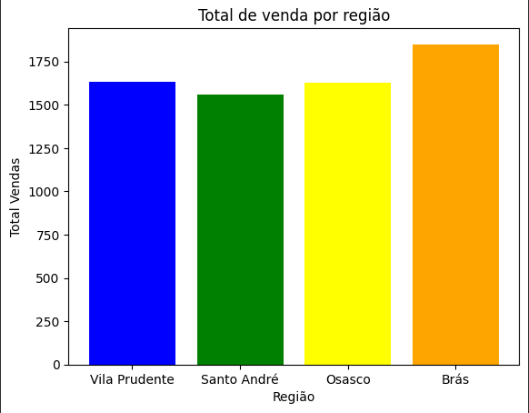
\includegraphics[width=1.0\linewidth]{figuras/Vendasregiao.png}
%     \caption{Enter Caption}
%     \label{fig:enter-label}
% \end{figure}




\section{Total de vendas por região}
\label{sec:figura}
A Figura~\ref{figuras/Vendasregiao.png} Após analisar gráfico, podemos ver que as vendas variam bastante de uma região para outra.
\begin{figure}[!ht]
	{\centering
		\caption{Descrição da figura.}
		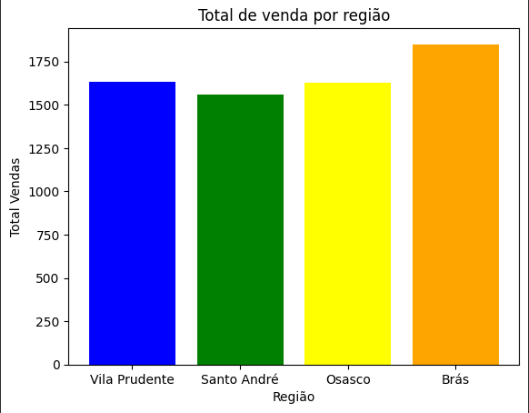
\includegraphics[width=1.0\textwidth]{figuras/Vendasregiao.png}
		\label{figuras/Vendasregiao.png}
		\fonte{Google Colab}
	}
\end{figure} \\ \\ \\ \\ \\ \\

\section{Total de vendas por regiaão selecionada}
\label{sec:figura}
A Figura~\ref{figuras/Total-vendas-produto-regiao.png} Após analise neste segundo gráfico, analisaremos qual é o produto mais vendido por cada região selecionada
\begin{figure}[!ht]
	{\centering
		\caption{Descrição da figura.}
		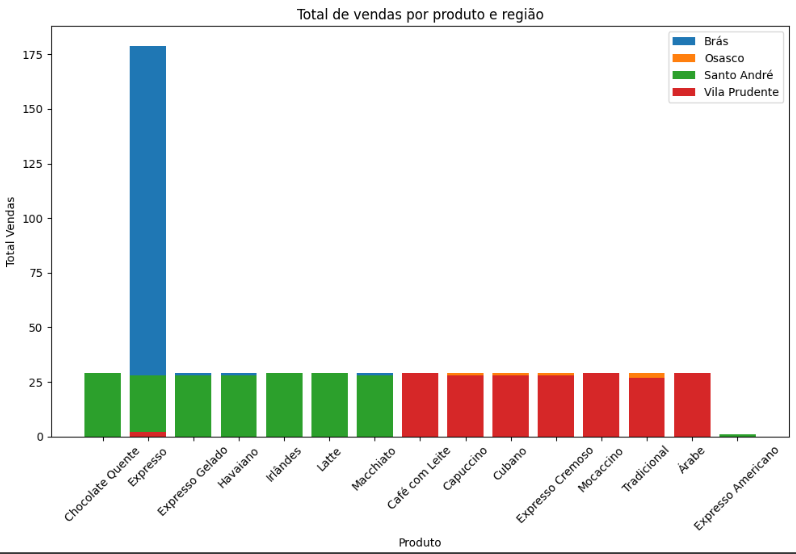
\includegraphics[width=1.0\textwidth]{figuras/Total-vendas-produto-regiao.png}
		\label{figuras/Total-vendas-produto-regiao.png}
		\fonte{Google Colab}
	}
\end{figure} \\ \\ \\ \\ \\ \\ \\ \\ \\ 

\section{Total de vendas por tipos de café na Vila Prudente. }
\label{sec:figura}
A Figura~\ref{figuras/Total-vendas-Vila-Prudente.png} Após analise neste terceiro gráfico, analisaremos qual é o produto mais vendido na região da Vila Prudente
\begin{figure}[!ht]
	{\centering
		\caption{Descrição da figura.}
		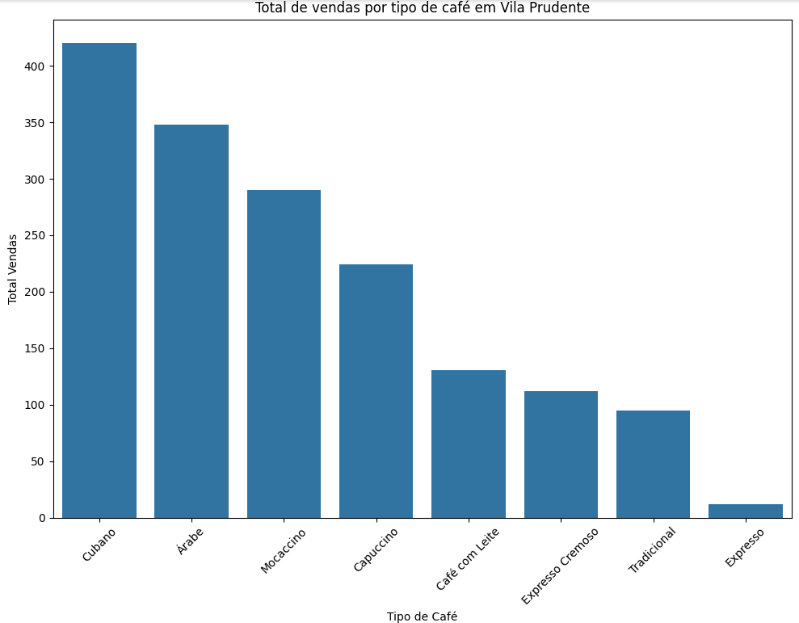
\includegraphics[width=1.0\textwidth]{figuras/Total-vendas-Vila-Prudente.png}
		\label{figuras/Total-vendas-Vila-Prudente.png}
		\fonte{Google Colab}
	}
\end{figure} \\ \\ \\ \\ \\ \\ \\ 

\section{Total de vendas por tipos de café em Santo André. }
\label{sec:figura}
A Figura~\ref{figuras/Total-vendas-Santo-Andre.png} Após analise neste quarto gráfico, mostrará qual é o café mais vendido na região de Santo André.
\begin{figure}[!ht]
	{\centering
		\caption{Descrição da figura.}
		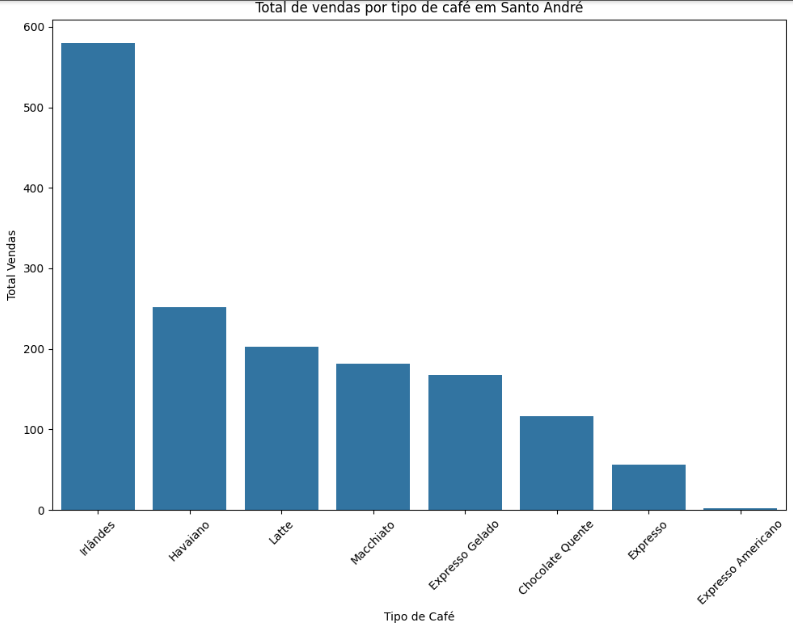
\includegraphics[width=1.0\textwidth]{figuras/Total-vendas-Santo-Andre.png}
		\label{figuras/Total-vendas-Santo-Andre.png}
		\fonte{Google Colab}
	}
\end{figure} \\ \\ \\ \\ \\ \\ \\ 

\section{Total de vendas por tipos de café em Osasco.}
\label{sec:figura}
A Figura~\ref{figuras/Total-vendas-Osasco.png} Após analise neste quinto gráfico, mostrará qual é o café mais vendido na região de Osasco.
\begin{figure}[!ht]
	{\centering
		\caption{Descrição da figura.}
		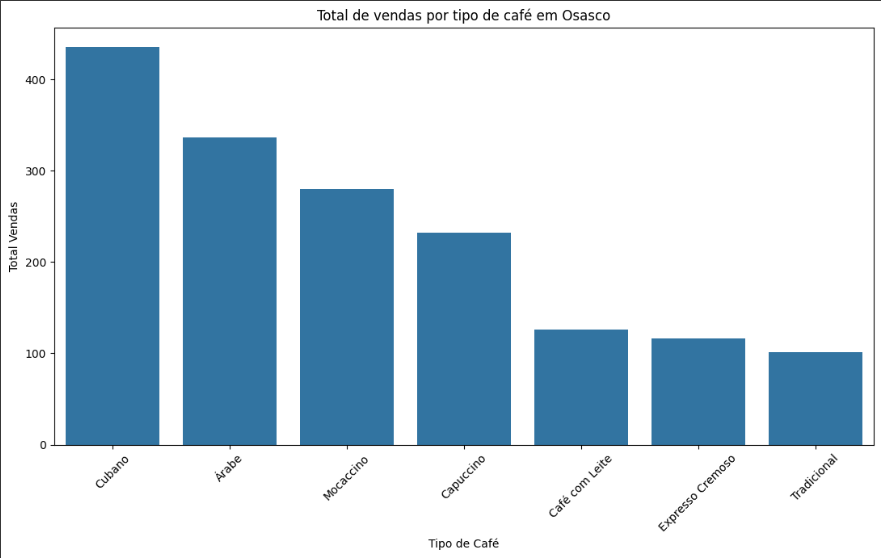
\includegraphics[width=1.0\textwidth]{figuras/Total-vendas-Osasco.png}
		\label{figuras/Total-vendas-Osasco.png}
		\fonte{Google Colab}
	}
\end{figure} \\ \\ \\ \\ \\ \\ \\ \\ \\ \\ 

\section{Total de vendas por tipos de café no Brás.}
\label{sec:figura}
A Figura~\ref{figuras/Total-vendas-Bras.png} Após analise neste sexto gráfico, mostrará qual é o café mais vendido na região do Brás.
\begin{figure}[!ht]
	{\centering
		\caption{Descrição da figura.}
		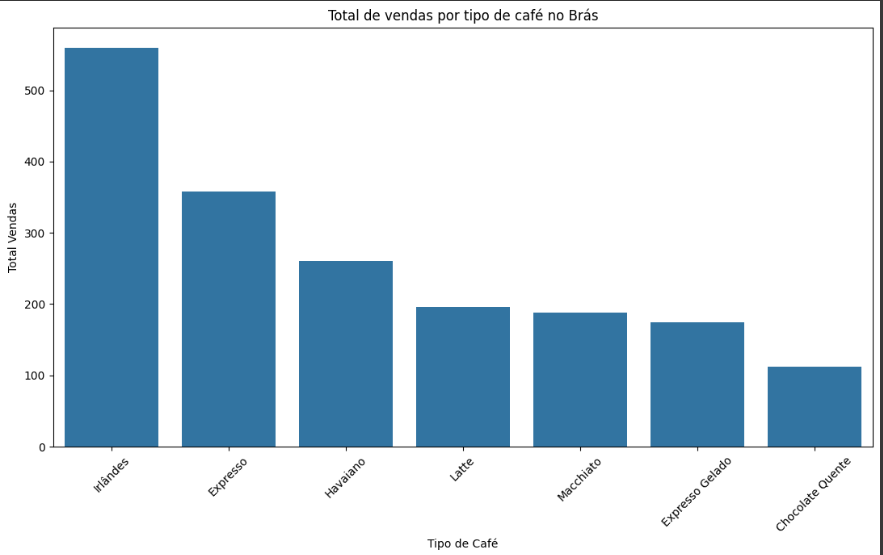
\includegraphics[width=1.0\textwidth]{figuras/Total-vendas-Bras.png}
		\label{figuras/Total-vendas-Bras.png}
		\fonte{Google Colab}
	}
\end{figure} \\ \\ \\ \\ \\ \\ \\ \\ \\ \\ \\ \\ 

\section{Analise de vendas de Café Expresso por Região.}
\label{sec:figura}
A Figura~\ref{figuras/Vendas-expresso-regiao.png} Após analise neste sétimo gráfico, mostrará o total de café expresso vendidos pelas regiões.
\begin{figure}[!ht]
	{\centering
		\caption{Descrição da figura.}
		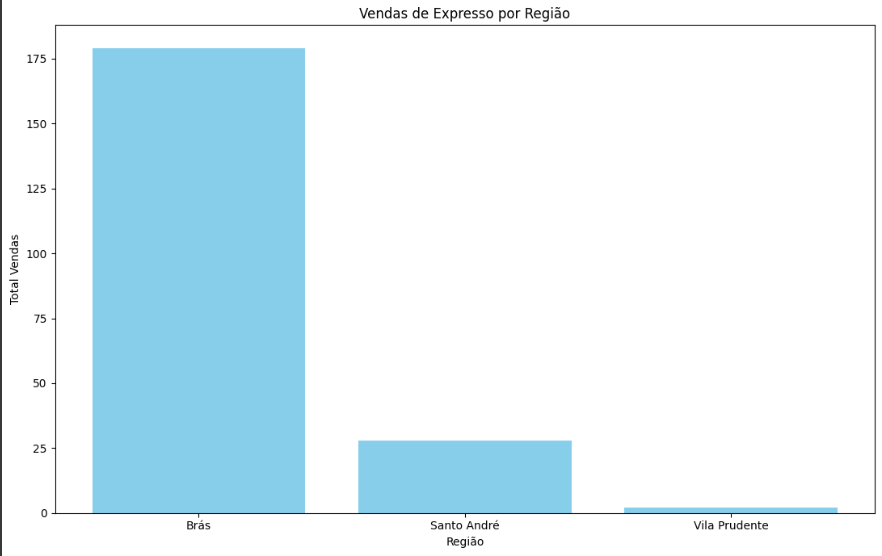
\includegraphics[width=1.0\textwidth]{figuras/Vendas-expresso-regiao.png}
		\label{figuras/Vendas-expresso-regiao.png}
		\fonte{Google Colab}
	}
\end{figure} \\ \\ \\ \\ \\ \\ \\ \\ \\  \\ \\ 

\section{Cafés mais vendidos por valores.}
\label{sec:figura}
A Figura~\ref{figuras/Cafe-mais-vendido-valor.png} Após analise deste oitavo gráfico, mostrará qual é o café mais vendido e o quanto eles renderam.
\begin{figure}[!ht]
	{\centering
		\caption{Descrição da figura.}
		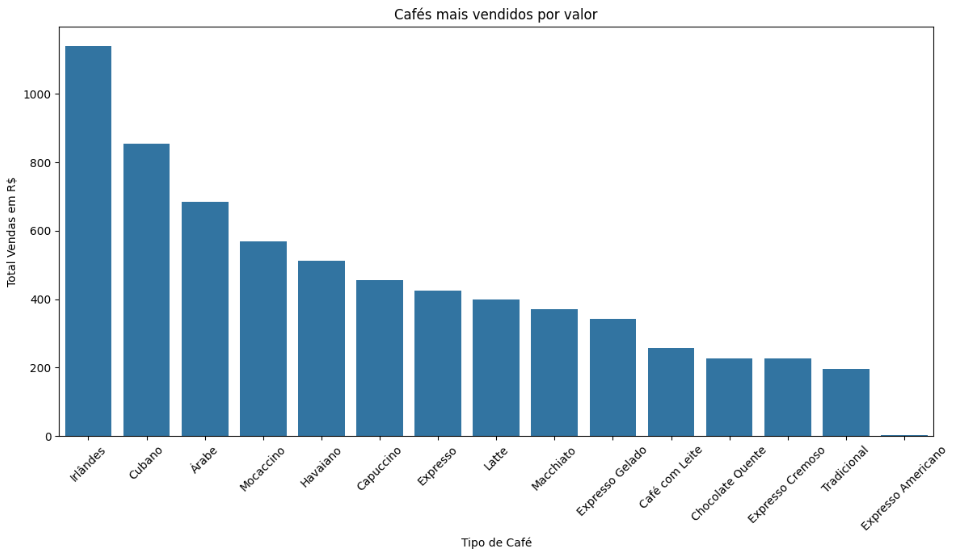
\includegraphics[width=1.0\textwidth]{figuras/Cafe-mais-vendido-valor.png}
		\label{figuras/Cafe-mais-vendido-valor.png}
		\fonte{Google Colab}
	}
\end{figure} \\ \\ \\ \\ \\ \\ \\ \\ \\ \\ \\ \\ \\ 

\section{Cafés mais vendidos por valor em cada região.}
\label{sec:figura}
A Figura~\ref{figuras/Cafe-mais-vendido-valor-cada-regiao.png} Ao investigarmos os cafés mais populares em cada região, mergulhamos no mundo dos gostos e preferências dos consumidores. Observamos não apenas números, mas também as histórias por trás de cada xícara.
\begin{figure}[!ht]
	{\centering
		\caption{Descrição da figura.}
		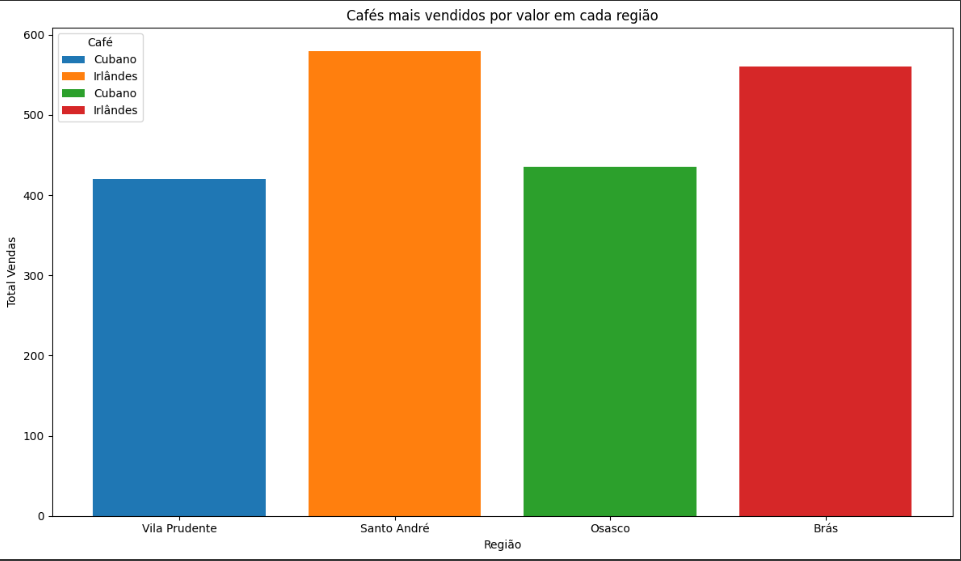
\includegraphics[width=1.0\textwidth]{figuras/Cafe-mais-vendido-valor-cada-regiao.png}
		\label{figuras/Cafe-mais-vendido-valor-cada-regiao.png}
		\fonte{Google Colab}
	}
\end{figure} \\ \\ \\ \\ \\ \\ \\ 




% \observacao{Observação/anotação para conversar com o orientador ou destacar importância.}

% Utilize o comando \texttt{$\backslash$tachado\{\}} para tachar um texto. Exemplo: \tachado{comprar} adquirir.

% Esse texto é um exemplo para \correcao{destaques de correção} a serem realizadas.

% \subsection{Subseção}
% \label{subsec:subseçao}
% Bla bla bla
